\chapter{Avaliação}
\label{chapter:avaliacao}

Este capítulo apresenta a campanha experimental formal, limitada a dez dias, executada no mesmo servidor para o G-FShield, os dois monólitos e um baseline com todas as características. A fonte única desta análise é o conjunto de resultados identificado pelo manifesto cujo SHA-256 é:
\begin{center}
\small\texttt{29fdc973ad6b243b297e34fcd539f5826aac4ce8a0870e8a5cea5caacfc9adc4}.
\end{center}
Os CSVs históricos de \texttt{tmp\_metrics/}, nos quais havia a divergência entre 25.873 linhas brutas e 25.836 linhas com F1 válido, não são combinados com a nova campanha. Assim, nenhuma dessas contagens é usada como resultado comparativo.

\section{Protocolo Experimental}

O corpus ERENO preservado possui 199.998 instâncias, 51 preditores e nove classes. Uma divisão estratificada, fixada antes das buscas com semente 20260825, produziu 119.998 instâncias de treino, 40.000 de validação e 40.000 de teste. Os hashes SHA-256 da origem, treino, validação e teste são, respectivamente, \texttt{60ebfcdc9c20}, \texttt{5876bf5570b7}, \texttt{c44a00ca554c} e \texttt{05d393c5881a}; os valores integrais constam do manifesto. O teste permaneceu indisponível para a busca e foi avaliado uma única vez depois da escolha da solução pela validação.

Todas as soluções finais foram reavaliadas pela mesma imagem com Weka J48 3.8.6, árvore podada, fator de confiança 0,25 e mínimo de duas instâncias por folha. A métrica primária é F1 macro na escala de 0 a 1; precisão e revocação macro, F1 ponderado, acurácia e F1 por classe foram preservados como medidas complementares.

A matriz possui 27 braços: 24 configurações distribuídas, dois monólitos e o baseline. Cada braço usa as sementes independentes 42--49, totalizando 216 execuções válidas. As configurações distribuídas cruzam quatro rankings da RCL (IG, GR, SU e ReliefF), dois controladores (VND e RVND) e três preferências iniciais de busca local (BF, IWSS e IWSSR). Os três operadores continuam habilitados no portfólio de cada controlador. ReliefF usa 1.000 instâncias de referência escolhidas de forma reproduzível no treino pela semente da execução; treino, validação e teste do classificador usam as divisões completas.

Cada execução algorítmica recebeu até 3.000 s, com reserva de 300 s para encerramento e avaliação final. A busca também poderia parar após 500 melhorias aceitas, considerando melhora mínima de 0,0001. O G-FShield usa corte 30, solução inicial de cinco atributos e 100 iterações por operador. O Monólito~1 executa GR seguido de Bit-Flip, com corte 30, cinco atributos e 100 iterações locais. O Monólito~2 executa GR seguido de IWSS sob VND, com os mesmos corte e tamanho inicial e 100 iterações locais. O baseline apenas treina e avalia J48 com os 51 preditores. Em cada caso, treino orienta o ajuste, validação escolhe a melhor solução e teste fornece a medida final comum.

Todos os braços foram confinados aos processadores lógicos 8--15 do nó NUMA~1, com teto agregado de oito CPUs e 16~GiB. Os contêineres foram amostrados a cada 30 s por \texttt{docker stats}; CPU corresponde à soma em núcleos e memória à soma dos contêineres pertencentes à execução. Outros contêineres presentes no host foram registrados separadamente e não entram nessas somas. A campanha começou em 25 de agosto de 2026 às 08:32 UTC e terminou em 1 de setembro de 2026 às 03:36 UTC, antes do limite de dez dias, sem reinício do supervisor.

Doze tentativas distribuídas terminaram sem solução completa (\path{NO_COMPLETE_SOLUTION}) e foram rejeitadas pelo contrato de artefatos. O orquestrador repetiu somente as combinações semente--braço ausentes até obter oito resultados válidos por braço. Foram, portanto, 228 tentativas e 216 execuções válidas. As 208 execuções de busca terminaram pelo limite de tempo; as oito execuções do baseline terminaram normalmente.

Neste capítulo, \emph{execução} é uma réplica válida e independente de um braço e uma semente. \emph{Solução final} é o subconjunto escolhido na validação e avaliado uma vez no teste. \emph{Registro interno} é uma linha ou evento de candidato produzido dentro dessa execução; registros internos são correlacionados e não são tratados como réplicas nem como soluções ponta a ponta.

\section{Qualidade Preditiva e Redução Dimensional}

A Tabela~\ref{tab:resultados-formais} resume a configuração G-FShield escolhida pelo maior F1 macro mediano de validação, os monólitos e o baseline. Para cada braço, as estatísticas usam oito execuções. RF--VND--IWSSR obteve F1 macro mediano de teste 0,9448, com intervalo interquartil 0,9441--0,9449, 11 atributos e redução de 78,4\%. O baseline com todos os atributos obteve 0,9378. A diferença mediana pareada foi 0,0069 em favor da configuração selecionada; trata-se de resultado descritivo, não de superioridade estatística demonstrada.

\begin{landscape}
\begin{table}[p]
\centering
\scriptsize
\caption{Resultados finais no teste reservado e recursos observados (medianas de oito execuções).}
\label{tab:resultados-formais}
\resizebox{.96\linewidth}{!}{%
\begin{tabular}{lrrrrrrrrrr}
\toprule
\textbf{Braço} & \textbf{F1 macro} & \textbf{Precisão} & \textbf{Revocação} & \textbf{Acurácia} & \textbf{$|S|$} & \textbf{Redução (\%)} & \textbf{Tempo (s)} & \textbf{CPU (núcleos)} & \textbf{RAM med. (MiB)} & \textbf{Pico RAM (MiB)} \\
\midrule
RF--VND--IWSSR & 0,9448 & 0,9463 & 0,9432 & 0,9343 & 11 & 78,4 & 2.815,3 & 2,104 & 4.726,0 & 5.858,3 \\
Monólito 1 (GR--BF) & 0,9397 & 0,9399 & 0,9396 & 0,9293 & 5 & 90,2 & 2.712,5 & 1,069 & 1.531,4 & 1.959,4 \\
Monólito 2 (GR--IWSS) & 0,8411 & 0,8571 & 0,8454 & 0,8412 & 5 & 90,2 & 2.725,9 & 1,003 & 1.394,7 & 1.788,9 \\
Todas as 51 características & 0,9378 & 0,9402 & 0,9358 & 0,9272 & 51 & 0,0 & 72,5 & 1,044 & 748,4 & 820,0 \\
\bottomrule
\end{tabular}}

\vspace{0.4em}
\parbox{.96\linewidth}{\footnotesize F1, precisão e revocação são macro. CPU é a mediana temporal da soma dos contêineres por execução e depois a mediana entre sementes. RAM mediana e pico seguem a mesma delimitação. O tempo é ponta a ponta, incluindo inicialização, busca, seleção por validação, encerramento controlado e avaliação final.}
\end{table}
\end{landscape}

O Monólito~1 obteve F1 mediano 0,9397; o Monólito~2 apresentou mediana 0,8411 e alta dispersão (média 0,7343; desvio-padrão 0,2013). O baseline é determinístico sob a configuração usada e repetiu 0,9378 nas oito sementes. Entre as 24 configurações distribuídas, o F1 mediano variou de 0,8671 a 0,9448; a mediana entre configurações foi 0,9418. Todas produziram oito subconjuntos finais distintos. O tamanho mediano variou de 5 a 17 atributos, equivalente a reduções de 90,2\% a 66,7\%.

\begin{figure}[p]
  \centering
  
\includegraphics[width=.94\linewidth,height=.80\textheight,keepaspectratio]{fig/gfshield/campaign-test-f1.pdf}
  \caption{Distribuição do F1 macro no teste para os 27 braços e oito sementes por braço.}
  \label{fig:campaign-test-f1}
\end{figure}

\begin{landscape}
\begin{figure}[p]
  \centering
  
\includegraphics[width=.96\linewidth,height=.80\textheight,keepaspectratio]{fig/gfshield/campaign-configuration-heatmap.pdf}
  \caption{F1 macro mediano no teste das 24 configurações distribuídas.}
  \label{fig:campaign-heatmap}
\end{figure}
\end{landscape}

A Figura~\ref{fig:campaign-heatmap} evidencia que as quatro combinações VND--BF permaneceram abaixo das configurações que efetivamente exploraram IWSS/IWSSR. Esse resultado depende do protocolo e do objetivo de busca implementado; não estabelece que um operador seja universalmente inferior. A relação entre qualidade e redução aparece na Figura~\ref{fig:campaign-quality-reduction}. RF--VND--IWSSR supera descritivamente o baseline em F1 com 40 atributos a menos, enquanto o Monólito~1 usa somente cinco atributos e preserva F1 próximo ao baseline.

\begin{landscape}
\begin{figure}[p]
  \centering
  
\includegraphics[width=.96\linewidth,height=.80\textheight,keepaspectratio]{fig/gfshield/campaign-quality-reduction.pdf}
  \caption{Compromisso entre F1 macro mediano e redução dimensional das soluções finais.}
  \label{fig:campaign-quality-reduction}
\end{figure}
\end{landscape}

O desempenho por classe (Figura~\ref{fig:campaign-per-class}) revela a informação ocultada pela média: para RF--VND--IWSSR, as medianas de F1 são 0,7179 em \textit{grayhole}, 0,8451 em \textit{normal} e pelo menos 0,9565 nas demais sete classes. Portanto, o F1 macro próximo de 0,945 não significa desempenho uniforme entre ataques.

\begin{landscape}
\begin{figure}[p]
  \centering
  
\includegraphics[width=.97\linewidth,height=.80\textheight,keepaspectratio]{fig/gfshield/campaign-per-class-f1.pdf}
  \caption{F1 mediano por classe no teste para a configuração distribuída escolhida na validação e os comparadores.}
  \label{fig:campaign-per-class}
\end{figure}
\end{landscape}

\section{Tempo, Recursos e Interpretação Estatística}

Como as 208 buscas terminaram pelo mesmo limite, o tempo mediano ponta a ponta ficou entre 2.706 e 2.847 s por configuração. Esses valores não demonstram convergência mais rápida. Nenhuma das 24 configurações distribuídas atingiu F1 interno $\geq 0{,}95$. A auditoria do commit que originou as imagens confirmou que esse escore interno já é F1 macro multiclasse; a rotina binária com \texttt{normalClass=0} estava desabilitada. Ainda assim, a campanha não preservou uma linha do tempo cumulativa equivalente para cada candidato dos dois monólitos: seus CSVs registram a duração individual da avaliação, não o instante desde o início da execução. Portanto, não se calcula uma comparação válida de tempo até o limiar a partir dessa campanha. Esse desfecho requer timestamps monotônicos comparáveis nos dois braços, avaliação apenas na validação e censura no mesmo prazo.

Sob o mesmo teto agregado, as execuções distribuídas usaram mediana global de 3,56 núcleos e pico mediano de 5,45, contra aproximadamente 1,07/1,83 no Monólito~1 e 1,00/1,82 no Monólito~2. A memória distribuída teve mediana global de 5.317~MiB e pico mediano de 6.757~MiB, contra picos medianos de 1.959 e 1.789~MiB nos monólitos. Isso quantifica consumo observado, mas não prova eficiência: o pipeline distribuído agrega vários processos Java e infraestrutura de mensageria, enquanto os braços comparados executam rankings e operadores de busca diferentes.

\begin{landscape}
\begin{figure}[p]
  \centering
  
\includegraphics[width=.96\linewidth,height=.80\textheight,keepaspectratio]{fig/gfshield/campaign-resources.pdf}
  \caption{CPU e memória observadas por arquitetura sob o teto agregado comum de oito CPUs e 16~GiB.}
  \label{fig:campaign-resources}
\end{figure}
\end{landscape}

Como análise exploratória, cada configuração distribuída foi comparada aos três comparadores por semente com teste exato bilateral de inversão de sinais e tamanho de efeito bisserial por postos. A correção de Holm foi aplicada separadamente à família de 24 comparações de cada comparador. Para RF--VND--IWSSR, houve sete vitórias e uma derrota diante do baseline e oito vitórias diante de cada monólito; os três valores $p$ ajustados foram 0,1875. Nenhuma das 72 comparações ajustadas ficou abaixo de 0,05. Com oito sementes, os intervalos e testes têm baixo poder; os resultados sustentam diferenças descritivas, não afirmações de significância ou causalidade arquitetural.

\section{Experimento Causal Pareado da Arquitetura}
\label{sec:architecture-causal}

Para separar arquitetura de algoritmo, uma segunda campanha comparou duas implementações da mesma sequência RF--VND--IWSSR: o pipeline G-FShield e um executável monolítico sequencial. Foram fixados a especificação dos operadores, Weka J48, função objetivo, divisões de dados, parâmetros, sementes, prazo de seleção de 2.700~s e teto agregado de seis CPUs e 12~GiB. O braço distribuído empregou três consumidores para permitir que uma construção prosseguisse enquanto outra solução estava em busca local; o monólito executou as mesmas fases em sequência. A ordem AB/BA foi balanceada entre as sementes 42--71. Como as implementações usam runtimes distintos, efeitos residuais de implementação não podem ser completamente excluídos.

O protocolo pré-especificou como desfecho primário o tempo censurado até F1 macro de validação $\geq 0{,}94$, com diferença pareada definida como distribuído menos monólito e teste de permutação unilateral. A interpretação favorável também exigia que o limite inferior unilateral de 95\% da diferença média de F1 macro no teste não fosse inferior a $-0{,}005$. Candidatos foram pontuados somente na validação; o teste reservado foi consultado uma vez para a solução final. A campanha terminou com 60 execuções válidas, ou 30 pares. Sete tentativas distribuídas anteriores falharam durante a inicialização de Kafka/ZooKeeper e foram rejeitadas e repetidas pelo contrato; nenhum dos 60 manifestos válidos apresentou erro de checksum.

\begin{landscape}
\begin{table}[p]
\centering
\scriptsize
\caption{Campanha causal: medianas por arquitetura e comparações pareadas em 30 sementes.}
\label{tab:architecture-causal}
\resizebox{.96\linewidth}{!}{%
\begin{tabular}{lrrrl}
\toprule
\textbf{Medida} & \textbf{G-FShield} & \textbf{Monólito} & \textbf{Diferença pareada mediana} & \textbf{Resultado} \\
\midrule
F1 macro no teste & 0,945529 & 0,944699 & $+0{,}000017$ & 15 vitórias, 10 empates, 5 derrotas \\
Tempo até F1 $\geq 0{,}94$ (s) & 940,077 & 701,255 & $+422{,}740$ & $p=0{,}000795$; distribuído mais lento \\
AUC \textit{anytime} normalizada & 0,879884 & 0,897069 & $-0{,}016898$ & $p_{Holm}=0{,}000055$ \\
Candidatos por segundo & 0,1074 & 0,0739 & $+0{,}0317$ & 30/30 pares; $p_{Holm}=0{,}000055$ \\
CPU mediana utilizada (núcleos) & 4,076 & 1,004 & $+3{,}070$ & 30/30 pares \\
CPU-h por candidato & 0,010875 & 0,003821 & $+0{,}007095$ & 0/30 pares favoráveis ao distribuído \\
GiB-h por candidato & 0,012366 & 0,004904 & $+0{,}007397$ & 0/30 pares favoráveis ao distribuído \\
Sobreposição construção--busca local & 99,998\% & 0\% & $+99{,}998$ p.p. & 30/30 pares; $p_{Holm}=0{,}000055$ \\
Redução dimensional & 78,43\% & 76,47\% & $+1{,}96$ p.p. & 18 vitórias, 12 empates; $p_{Holm}=0{,}000080$ \\
\bottomrule
\end{tabular}}
\end{table}
\end{landscape}

O desfecho primário contradiz a hipótese de menor latência para uma única requisição: o G-FShield demorou mais para atingir 0,94 em 23 dos 30 pares. A diferença média pareada de F1 no teste foi $-0{,}001759$, e o limite inferior unilateral de 95\% foi $-0{,}005615$; como ultrapassou por pouco a margem negativa pré-especificada de $-0{,}005$, a salvaguarda de não inferioridade também não foi satisfeita. O limiar 0,95 foi censurado em todos os pares e não distingue as arquiteturas.

Em contrapartida, a decomposição produziu o mecanismo arquitetural pretendido: praticamente toda a busca local ocorreu em paralelo à construção, enquanto a execução monolítica permaneceu sequencial. Isso elevou a vazão mediana de avaliações de candidatos em aproximadamente 45\%, mas exigiu cerca de quatro vezes mais CPU simultânea e maior custo de CPU e memória por candidato. A Figura~\ref{fig:architecture-speed-processing} mostra conjuntamente esses efeitos. Portanto, ``melhor'' é uma conclusão dependente do objetivo: o G-FShield é superior para paralelismo observável, vazão bruta e, neste protocolo, redução dimensional; o monólito é superior para latência até 0,94 e eficiência por unidade de recurso. Não se demonstrou superioridade global da arquitetura distribuída.

\begin{landscape}
\begin{figure}[p]
  \centering
  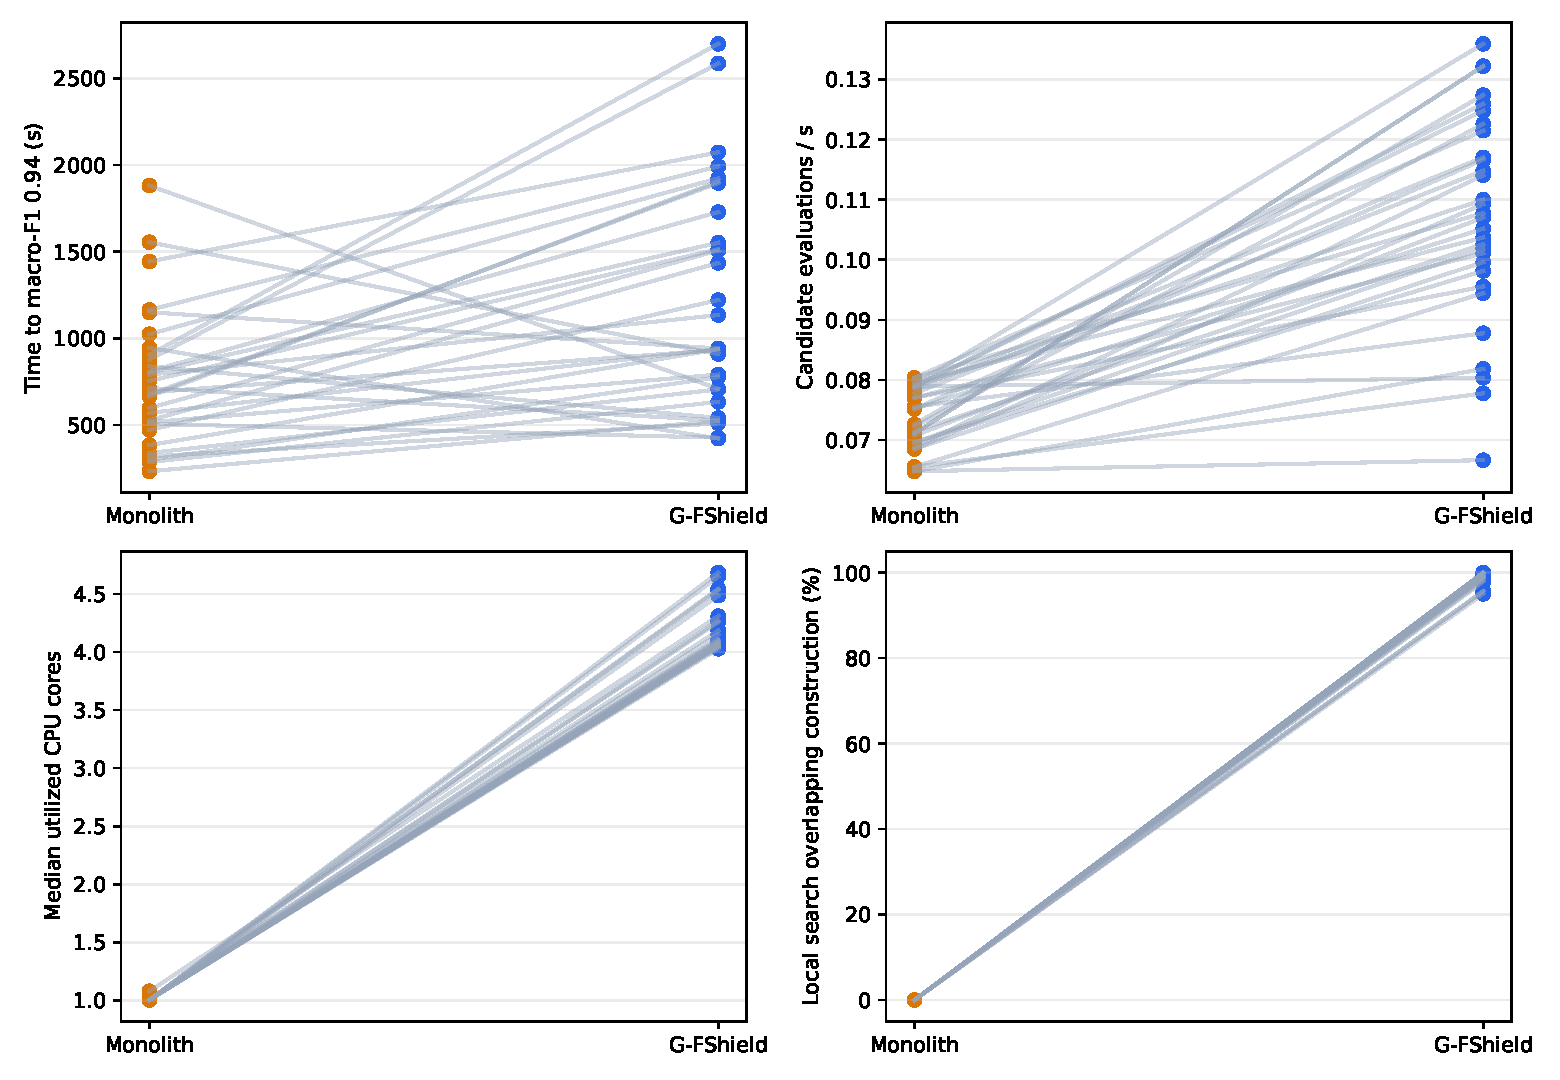
\includegraphics[width=.96\linewidth,height=.80\textheight,keepaspectratio]{fig/gfshield/architecture-speed-processing.pdf}
  \caption{Comparações pareadas de tempo até F1 macro 0,94, vazão de candidatos, CPU utilizada e sobreposição entre construção e busca local.}
  \label{fig:architecture-speed-processing}
\end{figure}
\end{landscape}

A trajetória mediana da melhor validação (Figura~\ref{fig:architecture-anytime}) explica o resultado: o monólito alcança cedo soluções boas, ao passo que a maior vazão distribuída não se converte automaticamente em progresso de qualidade. A inspeção posterior sugeriu contar subconjuntos \emph{distintos} com F1 de validação $\geq 0{,}945$ por prazo como uma medida de rendimento de soluções de alta qualidade. Como esse limiar foi escolhido após observar estes dados, ele não é usado como confirmação nesta campanha; foi congelado para uma nova campanha independente com sementes 72--101.

\begin{landscape}
\begin{figure}[p]
  \centering
  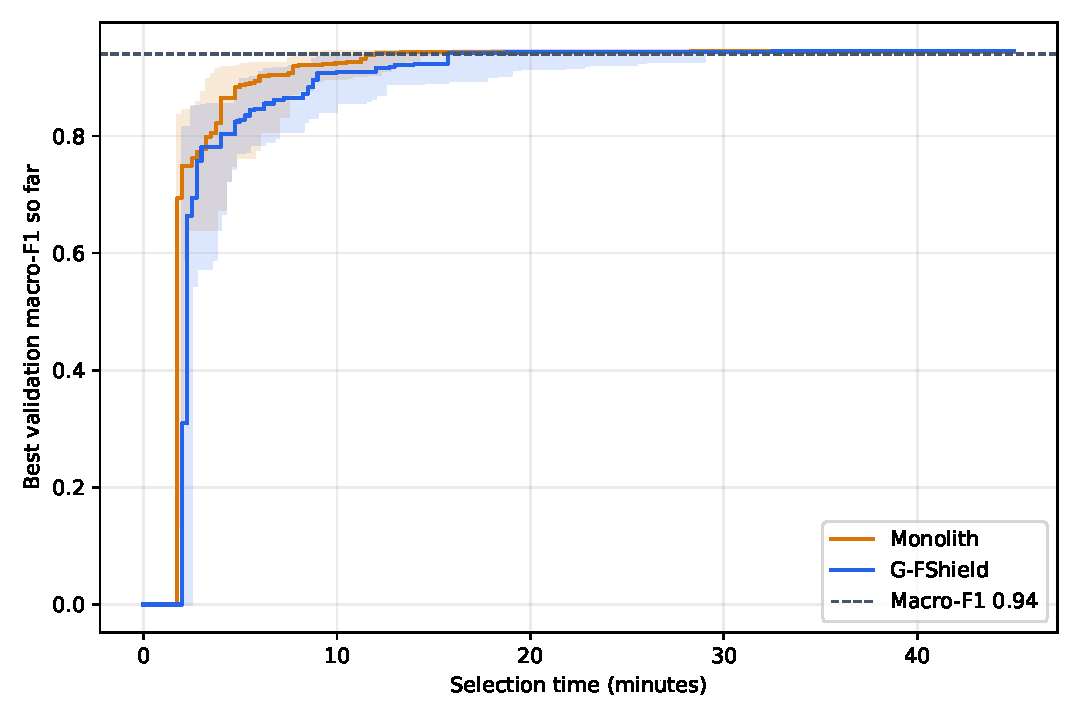
\includegraphics[width=.96\linewidth,height=.80\textheight,keepaspectratio]{fig/gfshield/architecture-anytime-validation-f1.pdf}
  \caption{Trajetória mediana da melhor solução na validação durante os 45 minutos de seleção. As faixas representam o intervalo interquartil entre sementes.}
  \label{fig:architecture-anytime}
\end{figure}
\end{landscape}

\section{Observabilidade e Rastreabilidade}

Cada execução preserva \texttt{campaign\_id}, \texttt{run\_id}, braço, semente, parâmetros, hashes dos dados, comando resolvido, estados, motivo de parada, timestamps UTC e monotônicos, solução selecionada, métricas finais, mensagens de melhor solução, CSVs internos, logs e telemetria de contêiner. Um manifesto de checksums por execução permite detectar alteração nos artefatos, e o estado da campanha permite reconstruir tentativas, rejeições e repetições.

Na aplicação, o backend persiste eventos de solução inicial, reinício de vizinhança, progresso de busca, solução refinada e melhor solução, além de tópico, partição, \textit{offset}, estado, \texttt{seedId}, timestamps e conteúdo JSON quando disponíveis. A campanha formal acrescenta \texttt{campaign\_id}, \texttt{run\_id} e \texttt{request\_id} aos fluxos experimentais, removendo a ambiguidade entre execuções concorrentes nesse protocolo. Ainda não foram medidos completude dos eventos, \textit{overhead} da instrumentação, perda/duplicação sob falha, tempo de recuperação ou sucesso de reprocessamento. Portanto, tolerância a falhas e resiliência permanecem objetivos de projeto.

\section{Ameaças à Validade}

\textbf{Validade interna.} Na primeira campanha, CPU, memória, conjunto de CPUs, dados, sementes, limite, J48 e F1 macro foram controlados, mas os comparadores executaram sequências algorítmicas distintas. O experimento causal posterior corrigiu esse confundimento, registrou trajetórias cumulativas equivalentes e balanceou a ordem AB/BA. Persistem possíveis efeitos de interferência do host compartilhado e de inicialização: 12 tentativas da primeira campanha e sete tentativas distribuídas da campanha causal foram rejeitadas e repetidas por não produzirem artefato completo. O procedimento preserva a matriz de sementes, mas condiciona a análise às execuções que inicializaram corretamente.

\textbf{Validade de construção.} A medida principal é F1 macro no teste reservado, e execução, solução final e registro interno foram separados. A escolha da mediana por braço reduz a influência de extremos, mas não resume toda a distribuição. CPU e memória medem contêineres, não energia nem custo monetário. O limiar 0,95 é convenção analítica, não requisito operacional.

\textbf{Validade de conclusão.} Na primeira campanha, oito sementes oferecem baixo poder, o baseline é determinístico e a escolha entre 24 configurações introduz seleção múltipla. No experimento causal, os 30 pares, o desfecho primário e a salvaguarda de qualidade foram definidos antes da análise; candidatos internos não foram tratados como réplicas. As medidas secundárias usam correção de Holm. A contagem de subconjuntos de alta qualidade proposta após a análise é explicitamente exploratória e requer confirmação nas sementes independentes 72--101.

\textbf{Validade externa.} A evidência cobre um servidor, um corpus IEC~61850, um particionamento e J48. Não demonstra generalização para outros corpora, classificadores, cargas concorrentes, números de réplicas, hardware, falhas ou ingestão contínua. Estudos posteriores devem repetir o protocolo com múltiplos conjuntos de dados e medir escalabilidade e recuperação separadamente.
